\documentclass[12pt]{article}

\usepackage[utf8]{inputenc}
\usepackage{graphicx}
\usepackage[portuguese]{babel}
\usepackage{float}

\title{MAC0344 Arquitetura de Computadores\\
Lista de Exercícios No. 2
}
\author{Mateus Agostinho dos Anjos\\NUSP 9298191}
\date{\today}

\begin{document}
	\maketitle
	\begin{itemize}
		\item[1 -]
			\hfill\\
			\begin{itemize}
				\item[a)]
					\hfill \\
					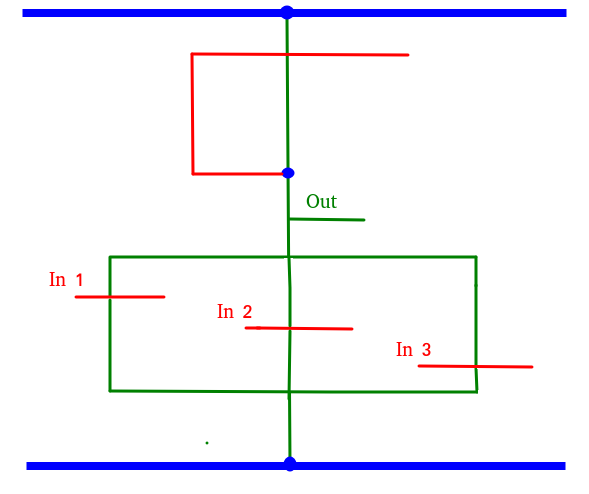
\includegraphics[width=5cm]{porta_NOR_3_entradas.png}
				\item[b)]
					\hfill \\
					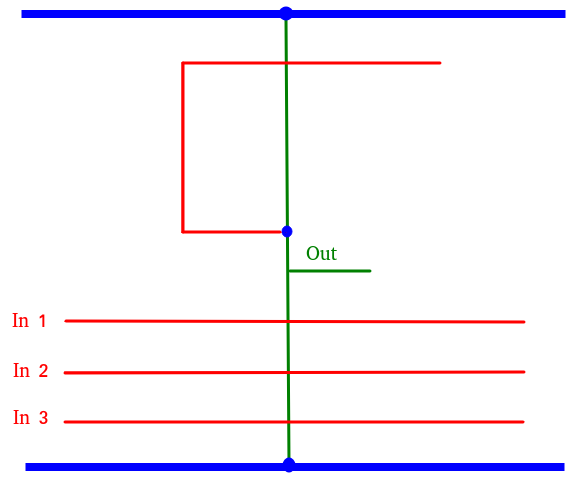
\includegraphics[width=5cm]{porta_NAND_3_entradas.png}
			\end{itemize}
		\item[2 -]
			Quando conduzindo eletricidade, o transistor MOS apresenta
			resistência efetiva de condução $r_{ef} = \alpha L/W$,
			portanto alternativa \textbf{(b)}.
		\item[3 -]
			A tecnologia do momento é \textbf{CMOS}, portanto
			alternativa \textbf{(b)}.
		\item[4 -]
			Seja $r_{efA} = \alpha L_A/W_A$ e $r_{efB} = \alpha L_B/W_B$.
			Como os transistores são do mesmo material, possuem o mesmo
			$\alpha$.\\
			Queremos:
			$$\frac{r_{efA}}{r_{efB}} = 8$$
			$$\frac{\alpha L_A/W_A}{\alpha L_B/W_B} = 8$$
			$$\frac{L_A/W_A}{L_B/W_B} = 8$$
			$$\frac{L_A}{W_A} = 8 * \frac{L_B}{W_B}$$
			Mantendo a mesma espessura W, para chegar no objetivo, devemos
			desenhar o transistor A com comprimento 8 vezes maior que
			B.\\
			Veja:
			\hfill \\
			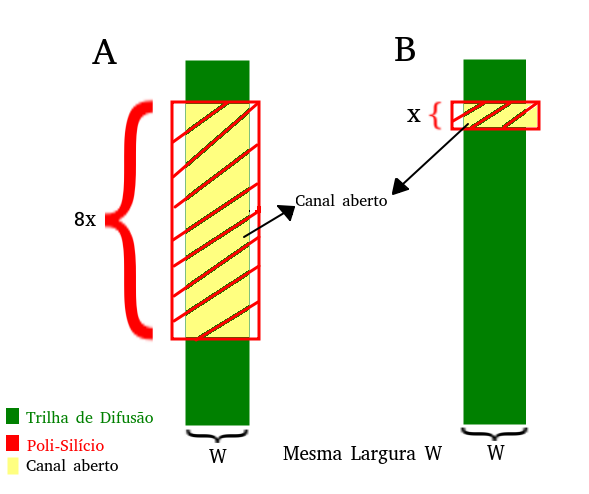
\includegraphics[width=12cm]{questao_4.png}
	\end{itemize}
\end{document}